\documentclass[a4paper, 11pt]{report}
\pdfpagewidth\paperwidth
\pdfpageheight\paperheight
\usepackage[english]{babel}
\usepackage[utf8]{inputenc}
\usepackage[T1]{fontenc}
\usepackage{amsmath,amssymb}
\usepackage{ esint }
\usepackage{ amssymb }
\usepackage{graphicx}
\usepackage{dsfont}
\usepackage{graphics}
\usepackage{float}
\usepackage{tipa}
\usepackage{amsthm}
\usepackage{subfigure}
\usepackage[write,infront,swapnames]{frontespizio}

\theoremstyle{definition}
\newtheorem{definition}{Definizione}[section]

\usepackage{sectsty}
\allsectionsfont{\centering \normalfont\scshape}


%%% Custom headers/footers (fancyhdr package)
\usepackage{fancyhdr}
\pagestyle{fancyplain}
\fancyhead{}											% No page header
\fancyfoot[L]{}											% Empty
\fancyfoot[C]{}											% Empty
\fancyfoot[R]{\thepage}									% Pagenumbering
\renewcommand{\headrulewidth}{0pt}			% Remove header underlines
\renewcommand{\footrulewidth}{0pt}				% Remove footer underlines
\setlength{\headheight}{13.6pt}


%%% Equation and float numbering
\numberwithin{equation}{section}		% Equationnumbering: section.eq#
\numberwithin{figure}{section}			% Figurenumbering: section.fig#
\numberwithin{table}{section}				% Tablenumbering: section.tab#


%%% Maketitle metadata
\newcommand{\horrule}[1]{\rule{\linewidth}{#1}} 	% Horizontal rule

\title{
		%\vspace{-1in}
		\usefont{OT1}{bch}{b}{n}
		\normalfont \normalsize \textsc{École Polytechnique Fédérale de Lausanne} \\ [25pt]
		\horrule{0.5pt} \\[0.4cm]
		\huge Analysis of students performances \\
		\horrule{2pt} \\[0.5cm]
}
\author{
		\normalfont 								\normalsize
        Bollero Francesco, Mariantoni Mattia, Mular Pau, Padovano Federica, Rossi Luca\\[-3pt]		\normalsize
        \today
}
\date{}


%%% Begin document
\begin{document}
\maketitle
\section{Introduction}
In this project we aimed to analyse a database containing information about a sample of students attending a Portuguese language course in two possible different schools ('Gabriel Pereira' or 'Mousinho da Silveira'). For each student there are different attributes related both to their academic performances and to their family context. The table in the next page describes what are the variables that we consider, we can notice that some of them are strictly related with the student academic life (for example "G1","G2","G3","absences" and "studytime") and others tend to describe the student social context, as the family (for example "famsize","Mjob" and "Fjob") and the social life.

\begin{figure}[h]\centering
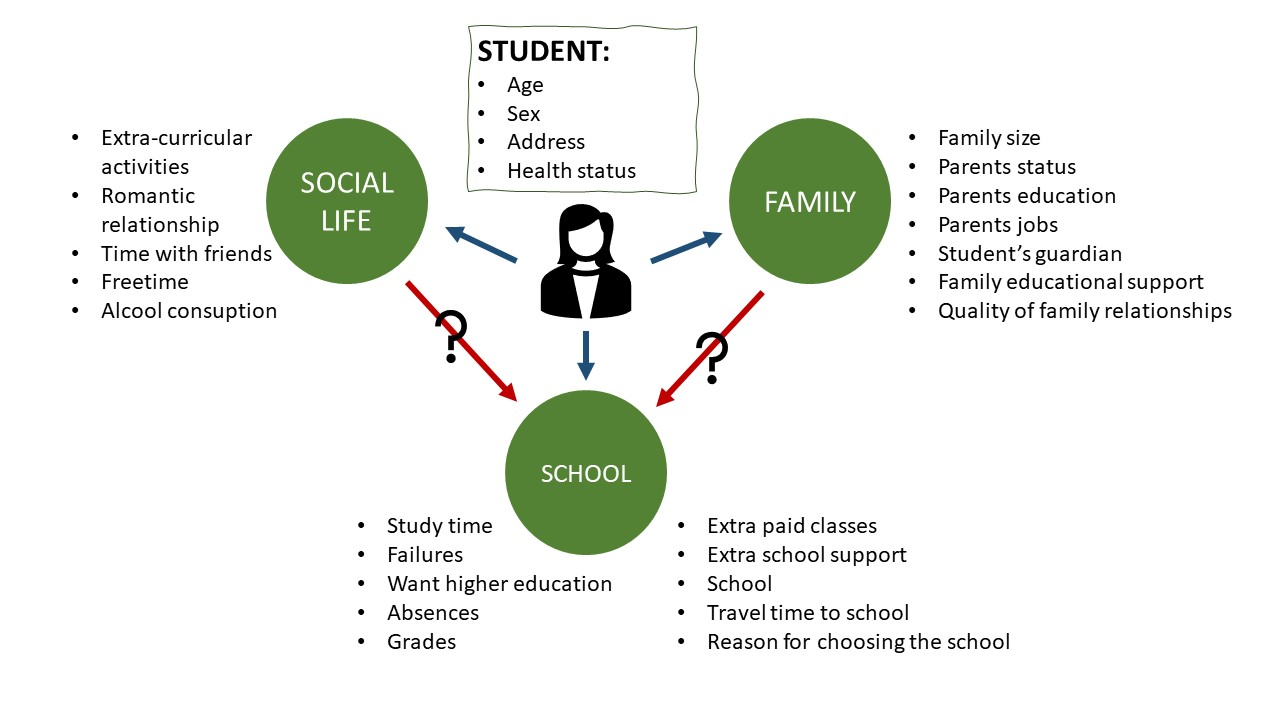
\includegraphics[scale=0.4]{variables.jpg}
\caption{Dataset variables associated with their macroarea.}
\end{figure}

\\After a first glance at the dataset these three variable subsets caught our eyes. In our opinion families and social life impact children's academic path in some way. There are many studies that show how parents with higher educational level have most likely children with higher grades or that want higher education. As the same time, we expect that someone who attends many extra-curricular activities and spend lots of time with friends has less time to study and therefore lower grades.
\\In this project we want to study the data in order to see if we can credit our opinions or not and to try to predict grades knowing all the other variables. For doing that we want to use statistical visualisations and statistical testing in order to give a more accurate and precise point of view of the analysis .


\flushleft
\noindent
\begin{figure}\makebox[1 \textwidth][c]{       %centering table
\resizebox{1.3 \textwidth}{!}{   %resize table
\begin{tabular}{ |p{2cm}|p{13cm}| }
\hline
Attributes &  Values\\
\hline
school & student's school (binary: "GP" - Gabriel Pereira or "MS" - Mousinho da Silveira)\\
\hline
sex & student's sex (binary: "F" - female or "M" - male)\\
\hline
age & student's age (numeric: from 15 to 22)\\
\hline
address & student's home address type (binary: "U" - urban or "R" - rural)\\
\hline
famsize & family size (binary: "LE3" - less or equal to 3 or "GT3" - greater than 3)\\
\hline
Pstatus & parent's cohabitation status (binary: "T" - living together or "A" - apart)\\
\hline
Medu & mother's education (numeric: 0 - none,  1 - primary education (4th grade), 2 – 5th to 9th grade, 3 – secondary education or 4 – higher education)\\
\hline
Fedu & father's education (numeric: 0 - none,  1 - primary education (4th grade), 2 – 5th to 9th grade, 3 – secondary education or 4 – higher education)\\
\hline
Mjob & mother's job (nominal: "teacher", "health" care related, civil "services" (e.g. administrative or police), "at_home" or "other")\\
\hline
Fjob & father's job (nominal: "teacher", "health" care related, civil "services" (e.g. administrative or police), "at_home" or "other")\\
\hline
reason & reason to choose this school (nominal: close to "home", school "reputation", "course" preference or "other")\\
\hline
guardian & student's guardian (nominal: "mother", "father" or "other")\\
\hline
traveltime & home to school travel time (numeric: 1 - <15 min., 2 - 15 to 30 min., 3 - 30 min. to 1 hour, or 4 - >1 hour)\\
\hline
studytime & weekly study time (numeric: 1 - <2 hours, 2 - 2 to 5 hours, 3 - 5 to 10 hours, or 4 - >10 hours)\\
\hline
failures & number of past class failures (numeric: n if 1<=n<3, else 4)\\
\hline
schoolsup & extra educational support (binary: yes or no)\\
\hline
famsup & family educational support (binary: yes or no)\\
\hline
paid & extra paid classes within the course subject (Math or Portuguese) (binary: yes or no)\\
\hline
activities & extra-curricular activities (binary: yes or no)\\
\hline
nursery & attended nursery school (binary: yes or no)\\
\hline
higher & wants to take higher education (binary: yes or no)\\
\hline
internet & Internet access at home (binary: yes or no)\\
\hline
romantic & with a romantic relationship (binary: yes or no)\\
\hline
famrel & quality of family relationships (numeric: from 1 - very bad to 5 -excellent)\\
\hline
freetime & free time after school (numeric: from 1 - very low to 5 - very high)\\
\hline
goout & going out with friends (numeric: from 1 - very low to 5 - very high)\\
\hline
Dalc & workday alcohol consumption (numeric: from 1 - very low to 5 - very high)\\
\hline
Walc & weekend alcohol consumption (numeric: from 1 - very low to 5 - very high)\\
\hline
health & current health status (numeric: from 1 - very bad to 5 - very good)\\
\hline
absences & number of school absences (numeric: from 0 to 93)\\
\hline
G1 & first period grade (numeric: from 0 to 20)\\
\hline
G2 & second period grade (numeric: from 0 to 20)\\
\hline
G3 & final grade (numeric: from 0 to 20, output target)\\
\hline
\end{tabular}
}
}
\caption{\label{fig:text3}Variables meaning}
\end{figure}


We also decide to split our work in four different points answering different questions:
\begin{enumerate}
\item What's the correlation between variables? Do the grades follow a normal distribution ?
\item Which is the capacity of different variables to explain the grades ?
\item Can we train a model to predict grade based on the other variables ?
\end{enumerate}
and for each point we used different statistical methods.


\section*{1. Correlations and Hypothesis testing}


\begin{itemize}
\item Correlation between Study time and Grades

\begin{figure}[h]\centering
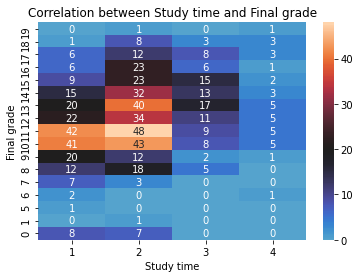
\includegraphics[scale=0.5]{g3-st.png}
\caption{Study times - Final grades.}
\end{figure}


\item Correlation between Sex and academic performances


\item Correlation between age and Final grade


\item Correlation between Student family and grades


\end{itemize}




\section*{1. Correlations and Hypothesis testing}

\section*{3. Grades}


\section*{4. Machine Learning}

All the models have been trained with a 80 to 20 percentage split for training to testing and implemented using the Sklearn library.

\subsection*{Baseline}
The baseline is a constant prediction model which outputs always the most frequent class ( in our dataset is 11 ), this achieves an accuracy of 16 percent.
\subsection*{Logistic Regression}
Logistic regression is a statistical model that in its basic form uses a logistic function to estimate the probabilities for a multivariate dependent variable: $$p=\frac{1}{1+b^{-\left(\beta_{0}+\beta_{1} x_{1}+\beta_{2} x_{2}+\cdots+\beta_{m} x_{m}\right)}}$$
Our model with L2 loss and balanced weights achieved an accuracy of 10.7 percent.
\subsection*{Random Forest}
Random forests are an ensemble learning method, used for classification in this case, that operates by constructing a multitude of decision trees at training time and correct for decision trees' habit of overfitting to their training set. Our model with max depth of a tree equal to 2 achieved an accuracy of 12.3 percent.
\subsection*{XGboost}
XGboost is a gradient boosting is a machine learning technique, used for classification in this case, which produces a prediction model in the form of an ensemble of weak prediction models, typically decision trees. In particular XGboost is also connected to the Newton-Raphson method. Our model with max depth of a tree equal to 3 achieved an accuracy of 23.8 percent.

\section*{4. Machine Learning}
The aim of the Machine Learning section is to apply some of the most popular Machine Learning techniques to our dataset in order to generalise relevant information contained in the dataset.
The easiest and first question which we want to address is the following:
\begin{itemize}
\item \textit{Can we build a model which can predict the final grade G3 based on the other features ?}
\end{itemize}
To answer this question we tried different models and we compared their performances. First of all, we preprocessed the data. Indeed, as we can see from the table above (which contains the information of the dataset) our original dataset is made of discrete and categorical features. For instance, the attribute 'address' is categorical because it can be 'U' for urban and 'R' for rural so it can belong to two distinct classes and there is no ordering relationship between the classes. However, we have also some variables which assume discrete range of values like 'age' which is a number from $15$ to $22$ or 'G1' which is an integer from $0$ to $20$. The first thing that we need to do is saving the dataset in a pandas dataframe and then perform one hot encoding on categorical variables. Indeed, for each categorical variable $v$ assuming values in a set $S$ with $S=\{s_1,s_2,\dots, s_k\}$, we create $k$ new columns and for each row we set the n-th created column equal $1$ if and only if in the original column v assumed the value $s_n$, we set it to zero otherwise, we finally delete the original column. In this way we are mapping each value $s_i$ to a vector with $k$ components whose i-th component is equal to one and the other components are equal to zero. This is a common technique in Machine Learning because it allows to encode categorical values in numerical values on the top of which we can train our machine learning model. Then we plot the correlation matrix to discover which variables are the most correlated to the output we would like to predict (G3). The result is shown below.
\begin{figure}[h]\centering
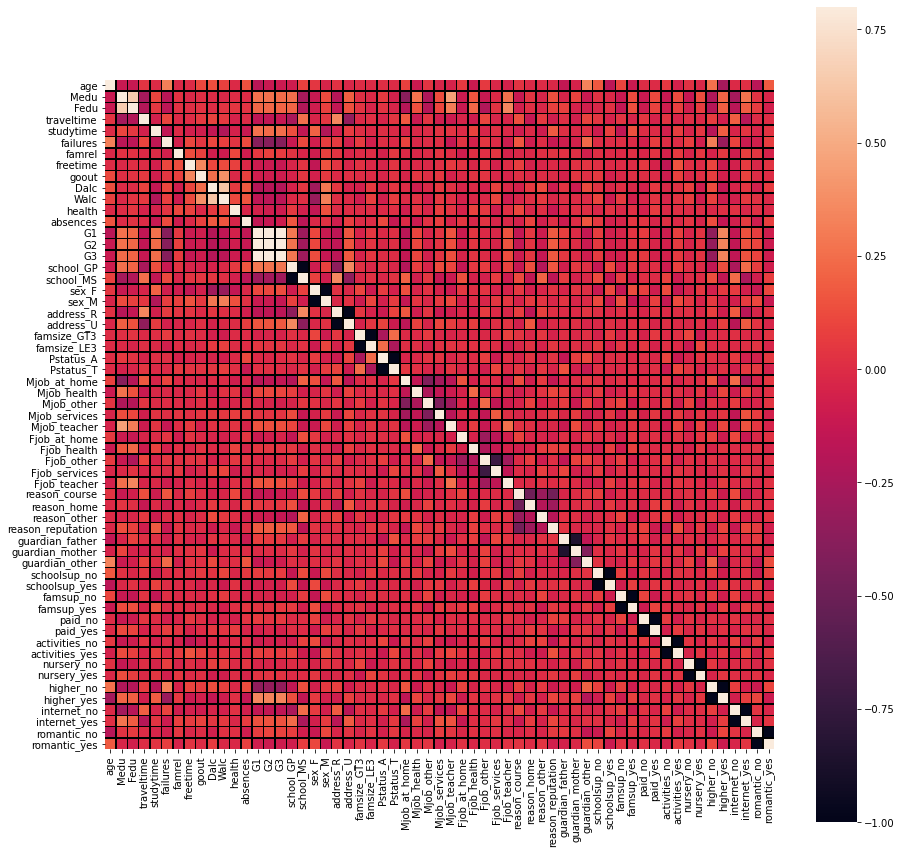
\includegraphics[scale=0.4]{heatmap.png}
\caption{Correlation between the variables of the preprocessed dataset}
\end{figure}
As we can easily observe, there is a high correlation between G3 and G1, G2, we have a low but significant positive correlation between G3 and the study time, the mother and father education and the desire of pursuing a higher education. On the other hand we have a negative correlation between G3 and the number of failures, the number of workday/weekend alchool consumption and the desire not to pursue a higher education. All this information are exactly what we would have expected. Then we split the data in $X$, a matrix containing all the features a part from G3 and $Y$ a column vector containing just the G3 feature. We then split each of them in $X_{\text{train}}$, $X_{\text{test}}$, $Y_{\text{train}}$, $Y_{\text{test}}$. We will use $X_{\text{train}}$ and $Y_{\text{train}}$ to train our model and then we will evaluate the performance using $X_{\text{test}}$ and $Y_{\text{test}}$. To answer this question we have considered the problem as a regressive problem and we have used the following models/approaches.
\begin{enumerate}
    \item We used a dense Neural Network with 7 layers with a large number of neurons for each layer. We used 'relu' as the activation function and we chose Adam as the optimizer. In addition to that, in order to prevent overfitting we applied the following early stopping technique. We have taken a subset of the training data as validation data and at the end of each epoch we computed the loss that the current model would have had on the validation data and we have saved the model corresponding to the smallest validation loss. After we have trained our model, we applied the model to $X_{\text{test}}$ in order to obtain the predictions corresponding to $Y_{\text{test}}$ we then have rounded the predictions because G3 has to be an integer value between 0 and 20. We computed the Mean Squared Error between the predicted and the ground-truth grades and we have obtained a value of $1.94$. This information is not enough for us to understand if the model made a good fit or not for G3. Therefore, we tried to visualise the results obtained.
    This is how our results look like compared to the real grades.
    \begin{figure}[h]\centering
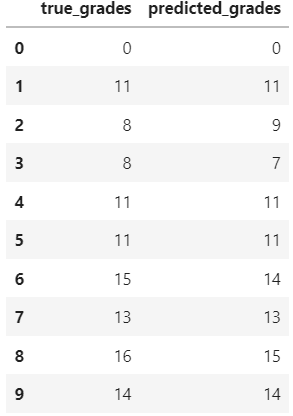
\includegraphics[scale=0.4]{predictions G3 neural nets using all features.PNG}
\end{figure}
As we can see from the first 10 students the predictions are quite accurate, however we cannot really understand how good the predictions are just comparing the true grades and the predicted grades with a table. We will now use different plots to have a better perspective of the fit. The first plot is a scatter plot of the true and predicted grades.
    \begin{figure}[h]\centering
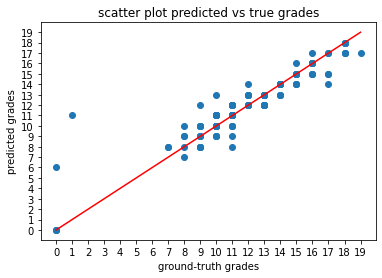
\includegraphics[scale=0.4]{scatter plot G3 neural nets using all features.png}
\end{figure}
We would expect the points to be on the line y=x since our predicted grades should be equal to the true grades. As we can see from the plot this is indeed true but of course not all the points lie on the line and some variance around the line is observed. We then used the following line plot to compare the predictions with the true grades for the first 20 students.
    \begin{figure}[h]\centering
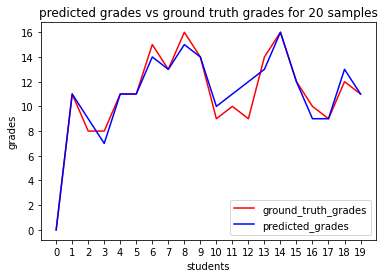
\includegraphics[scale=0.4]{plot G3 neural nets using all features.png}
\end{figure}
Again we observe that the predictions are quite accurate.
All this plots suggested a good fit but in order to confirm our hypothesis we have used the Kolmogorov-Smirnov test for goodness of fit. Having as a null hypothesis that the distributions of the true grades and the one of the predicted grades were the same distribution we obtained a very large p-value suggesting us that we cannot reject the null hypothesis and consequently that our fit is a good one.
\item As a second model we have used the support vector machine for regression. We have tuned the hyperparameters of the model using grid-search trying out different kernels, degree and coefficients. This model showed a worse performance compared to neural nets, indeed the Mean Squared Error in this case turned out to be $2.11$. The plots reflect the drop in performance.
\newline
    \begin{frame}
      \centering
        \begin{tabular}{c}
         \\
        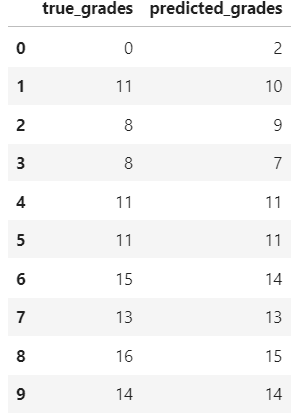
\includegraphics[width=4cm]{predictions G3 SVR using all the features.PNG}
      \end{tabular}

      \vspace{0.05em}
        \begin{tabular}{cc}
          &  \\
        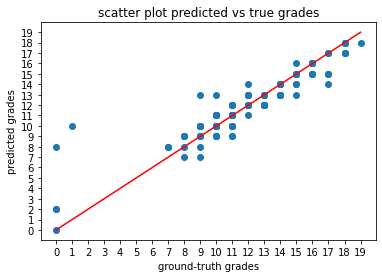
\includegraphics[width=4cm]{scatter plot G3 SVR using all the features.png}
         &
         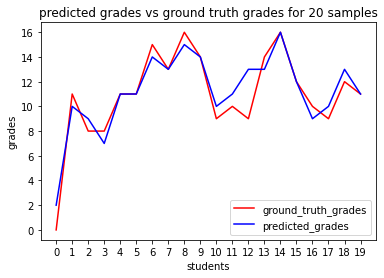
\includegraphics[width=4cm]{plot G3 SVR using all features.png}
         \end{tabular}
    \end{frame}
\newline
However, in this case too, we cannot reject the null hypothesis that the predicted grades and the true grades come from the same distribution using Kolmogorov-Smirnov test for goodness of fit.
\newline
\item To further increase the performance we can now train the neural net model on the same dataset but preprocessed such that no outliers are now present in the dataset. In this case we reach a mean squared error of 0.22 and as we can see the predicted grades are almost always correct.
\newline
    \begin{frame}
      \centering
        \begin{tabular}{c}
         \\
        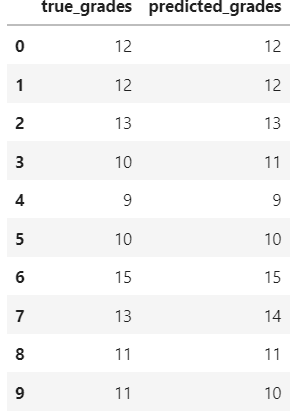
\includegraphics[width=4cm]{predictions G3 neural nets no outliers.PNG}
      \end{tabular}

      \vspace{0.05em}
        \begin{tabular}{cc}
          &  \\
        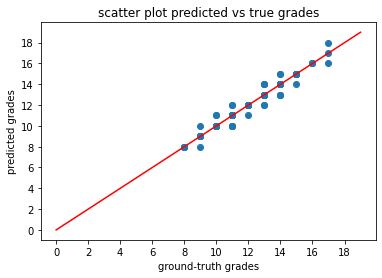
\includegraphics[width=4cm]{scatter plot G3 neural nets no outliers.png}
         &
         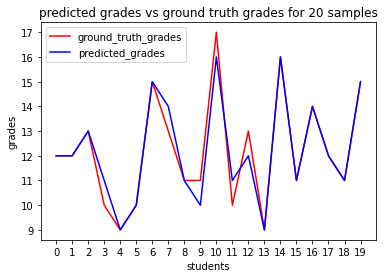
\includegraphics[width=4cm]{plot G3 neural nets no outliers.png}
         \end{tabular}
    \end{frame}
\newline
Clearly also in this case we cannot reject the null hypothesis of the Kolmogorov-Smirnov test for goodness of fit having a p-value of $0.9999999$.
\end{enumerate}
As we have seen our models work quite well and we can be satisfied of the reached fit. The next questions that might arise spontaneously is the following
\begin{itemize}
    \item \textit{Can we train a model which can predict the final grade G3 based on all the other features except the previous grades G1 and G2 ?}
\end{itemize}
We have tackled this question training the neural net model on a new $X'_{\text{train}}$ which is exactly the same as the $X_{\text{train}}$ described before a part from the column related to G1 and G2 which are not present in $X'_{\text{train}}$. The same applies to $X'_{\text{test}}$. We followed the exact same procedure described in the answer to the previous question but in this case we have reached a mean squared error of just $11.02$. The following plots testify this poor results.
\newline
    \begin{frame}
      \centering
        \begin{tabular}{c}
         \\
        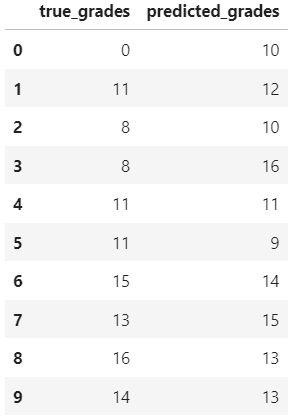
\includegraphics[width=4cm]{predictions G3 without G1 and G2.PNG}
      \end{tabular}

      \vspace{0.05em}
        \begin{tabular}{cc}
          &  \\
        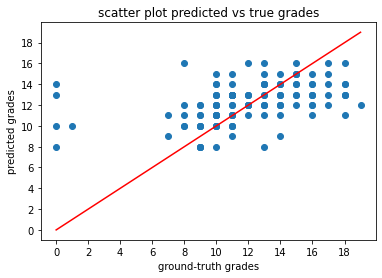
\includegraphics[width=4cm]{scatter plot G3 without G1 and G2.png}
         &
         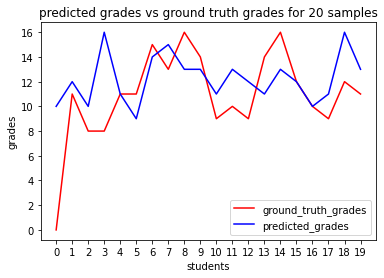
\includegraphics[width=4cm]{plot G3 without G1 and G2.png}
         \end{tabular}
    \end{frame}
\newline
As we can see from the scatter plot there is a high variety in the difference between the predictions and the true grades and how can we see in the line plot this drives to a poor fit. Also the Kolmogorov-Smirnov test notice the poor fit and now the p-vaue for the null hypothesis is only $0.067$. This does not indicate that we should reject the null hypothesis (with a significance level $\alpha = 0.05$) but it is an indicator of the poorness of the fit (since the p-value is quite small).
We could justify the results using the correlation matrix plotted before. Indeed, how we can see, G3 are highly positive correlated with G1 and G2 so, removing this two information, the model cannot predict G3 as well as before.
The next question that we are going to address is the following:
\begin{itemize}
    \item \textit{Can we predict the studytime based on the other features of the dataset ?}
\end{itemize}
We are going to answer to this question using a neural network based model since the best results obtained in the previous tasks were reached with this model. Obviously in this case after having split the dataset in training and test, $Y_{\text{train}}$ will be just the column related to the studytime and $X_{\text{train}}$ the columns for all the other features. The same applies to $X_{\text{test}}$ and $Y_{\text{test}}$. In this case when we apply the model to $X_{\text{test}}$ creating the prediction and when we compare them with $Y_{\text{test}}$ we have the following results.

\begin{figure}[h]\centering
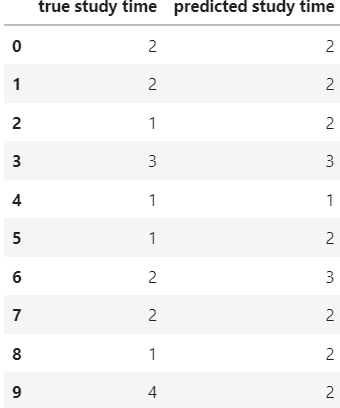
\includegraphics[scale=0.4]{prediction study time neural nets.PNG}
\end{figure}
    \begin{figure}[h]\centering
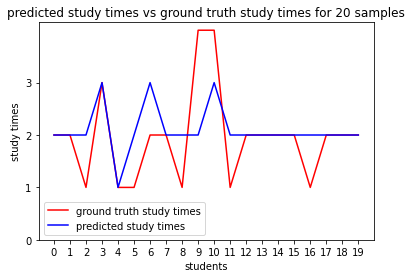
\includegraphics[scale=0.4]{plot study time neural nets.png}
\end{figure}

We have obtained another poor fit testified by a really small p-value in Kolmogorov-Smirnov test (0.0042). The reason why we have such a bad fit lies probably on the fact that we do not have enough data correlated with the feature 'studytime'. Indeed, the dataset was collected to explain the grades of the students and not their studytime. As a direct consequence, despite the model we use to predict the studytime, we will never have a good fit due to the lack of crucial missing variables such as the time that students spend at home or in different other activities.
The last question that we would like to give an answer to is the following:
\begin{itemize}
    \item \textit{Can we predict whether a student is in a romantic relationship or not based on the other features of the dataset?}
\end{itemize}
We have used three different models to answer to this question.
\begin{enumerate}
    \item A first method based on dense neural networks which scored $0.62$ in accuracy
    \item A second method based on Support Vector Machine tuned with grid-search which scored $0.65$ in accuracy
    \item A third model based on Logistic Regression tuned with grid-search which scored $0.65$ in accuracy.
\end{enumerate}
Recalling the definition of accuracy:
\begin{align*}
    \text{accuracy} = \frac{\text{number of correctly classified samples}}{\text{number samples}}
\end{align*}
we notice that an accuracy around $0.65$ is not high at all. Since we tried different models and we have always tuned the hyperparameters, we can claim that the problem lies in the lack of crucial variables as happened in the studytime analysis. Indeed, as we can observe from the correlation matrix, there are not highly positive or highly negative correlated variables with the romantic relationship variable.


% Pau's code starts
\newpage
\section{Explaining Academic Performance with Linear Regression}
The goal of this section is to find which factors determine the grade of a student. This is similar to what we did in section 2 with hypothesis testing, but now we also want to quantify the contribution of each variable and how they interact between them to explain the grades. We take the grade of the third semester as the response and the rest as explanatory variables. We assume that the underlying model is linear with a Gaussian response. We justify this choice in the model diagnosis and testing goodness of fit. For the time being, the use of linear models is motivated by their high interpretability despite not having as much predicting power as more complex models. \bigskip

We begin by removing the students that have a 0 in one of the grades. This decision is justified by the fact that in most education systems around the world is not possible to get a 0. Therefore it may not be a real grade but simply caused by the student moving to another school for example.  Removing these entries will have little impact on our capabilities to explain the data because there are only 17 students in this situation. Now we can have a first look at the data.\bigskip
\begin{center}
\begin{tabular}{ |c|c|c|c|c|c|  }
 \hline
 \multicolumn{6}{|c|}{3rd Semester Grades} \\
 \hline
\textbf{Min} & \textbf{1st Quart} & \textbf{Median} & \textbf{Mean} &  \textbf{3rd Quart} & \textbf{Max}\\
\hline
 5   & 10   & 12 &  12.21 &14&   19\\
 \hline
\end{tabular}
\end{center}
\bigskip In the following boxplot we can appreciate the symmetry of both the median and maximal values with respect to the IQR.
\begin{figure}[h]\centering
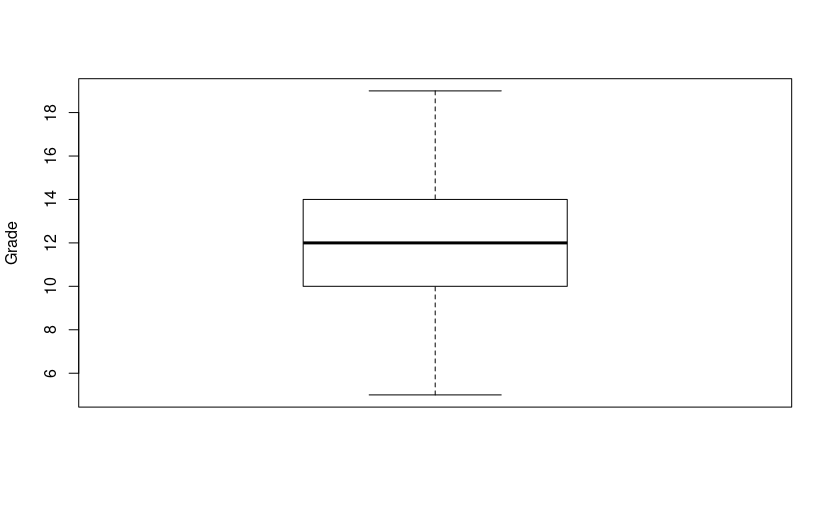
\includegraphics[width=0.75\textwidth]{pau1.png}
\caption{Final grades}
\end{figure}
\newpage
To understand in more detail how the grades are distributed we can look again at the histogram and  its corresponding smoothed density. \bigskip
\begin{figure}[h]\centering
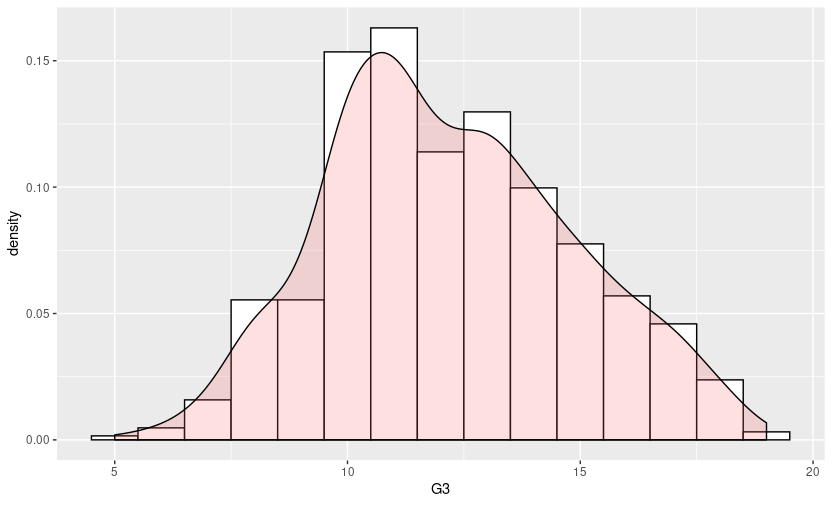
\includegraphics[width=0.9\textwidth]{pau2.png}
\end{figure}
If we want to find out how to combine the different input variables to predict the final grade it is crucial to understand the individual effect that each one has in the response variable.
\begin{figure}[h]\centering
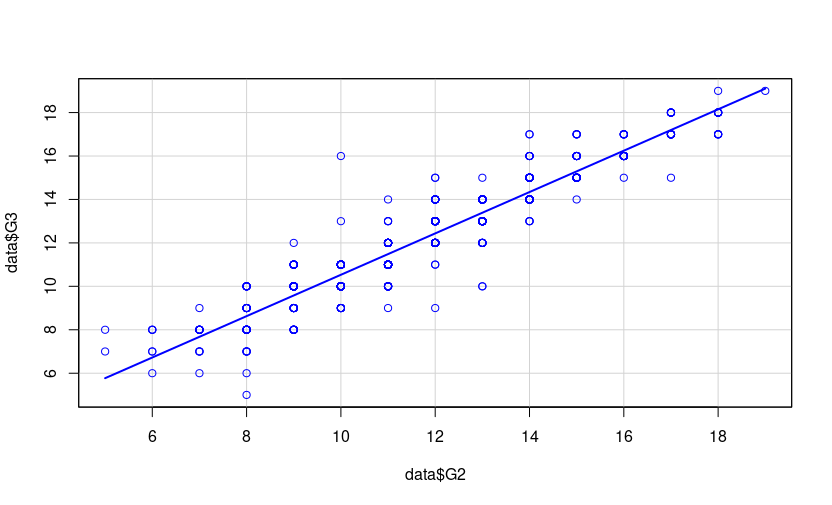
\includegraphics[width=0.9\textwidth]{pau3.png}
\caption{Scatterplot of the grade in the second term against the final grade}
\end{figure}
\newline
We can see that the grade in the second term explains quite well the final grade. Indeed, in most cases the final grade lies in the range of $\pm 3$ with respect to the second term grade. However, although the general trend is captured by the second term grade we also want to understand which factors contribute to increase/dicrease the grade with respect to the second term in order to explain the $\pm 3$ changes. If we are able to identify categorical variables which have either a positive or negative contribution to the final grade we will be able to better explain this changes. In fact the corresponding intercepts of those different groups would help to fit not only the scale but also the location.
Finally it is important to clarify why the points are vertically aligned. This is due to the fact that both variables (G2, G3) only take integer values. However when fitting the data we assume that they take real values because then we can express more accurately how sure is the model about the predicted value. For instance, either if the model outputs 13.9 or 13.5 our predicted grade will be 14, but the uncertainty will be much higher in the second case.\bigskip

\begin{figure}[h]\centering
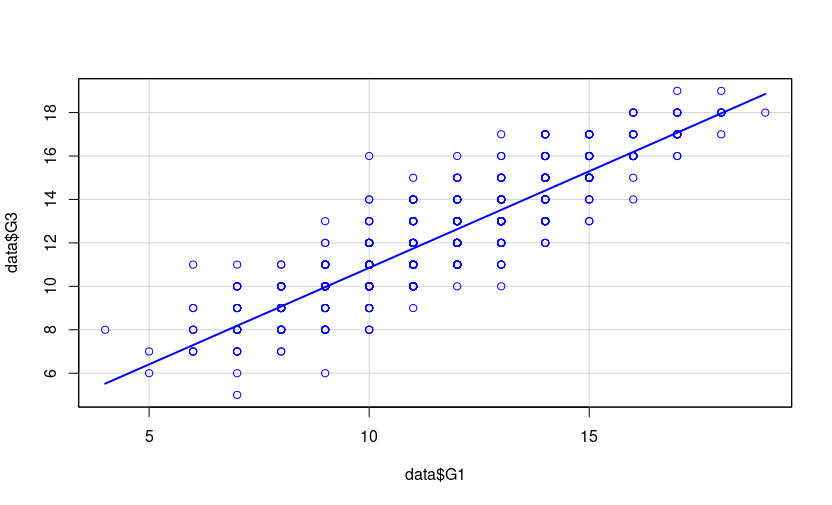
\includegraphics[width=0.9\textwidth]{pau4.png}
\caption{Scatterplot of the grade in the firs term against the final grade}
\end{figure}
\newline
As expected the effect of the first term grade on the final grade is very similar to the one exposed before for the second term grade. Moreover we can appreciate that the location changes are even bigger now. The higher uncertainty can be explained by the longer time interval between the grades. Therefore it is clear that we need to add some categorical variables that can capture this location changes. In a first step we want to visualize how does the final grade distribution changes among different groups defined from a categorical variable. In order to do so we compare the boxplots and smoothed densities of the final grade for different values of each categorical variable.
\newpage
\begin{figure*}[h]
\centering
\textbf{Sex}\par\medskip
\makebox[\linewidth][c]{%
\centering
\subfigure[Smoothed densities]{\label{fig:a}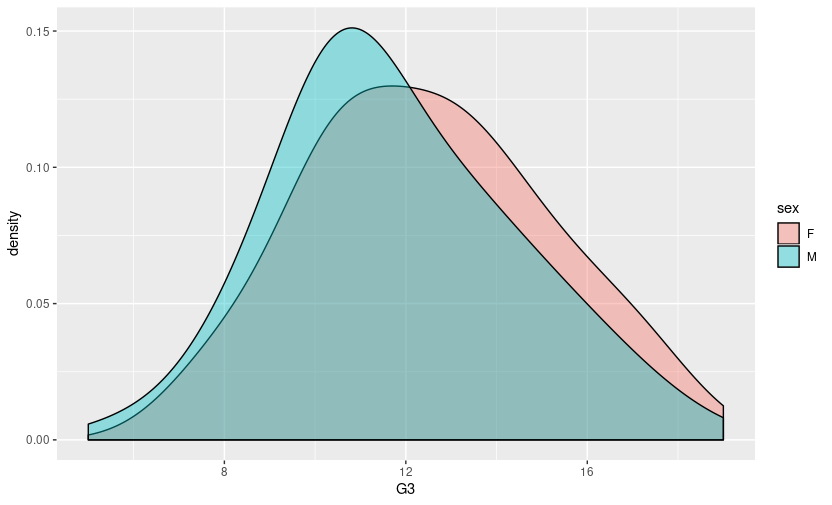
\includegraphics[width=0.6\textwidth]{pau6.png}}%
\subfigure[Boxplots]{\label{fig:b}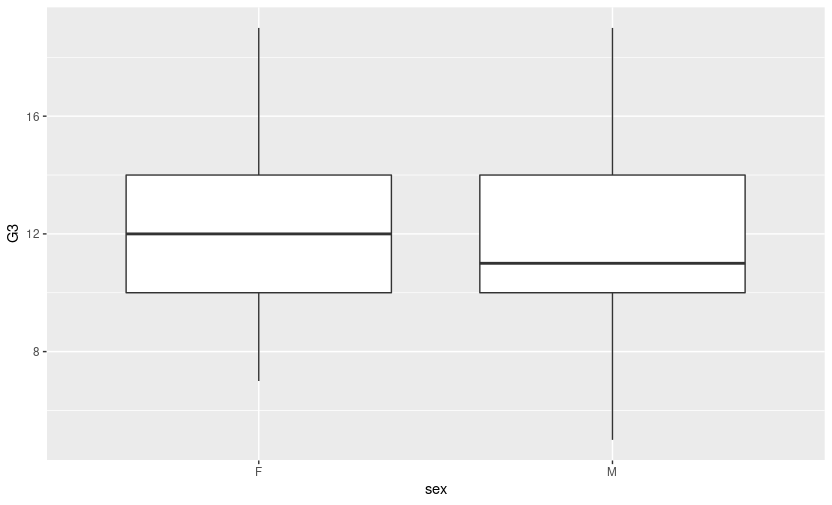
\includegraphics[width=0.6\textwidth]{pau7.png}}%
}
\end{figure*}
We can see that females tend to get better grades than males in our population. However the interquantile range looks exactly the same for both groups. The main difference relies on the median which is centered for females but positively skewed for males.\\[0.4in]
\begin{figure*}[h]
\centering
\textbf{Higher Education}\par\medskip
\makebox[\linewidth][c]{%
\centering
\subfigure[Smoothed densities]{\label{fig:a}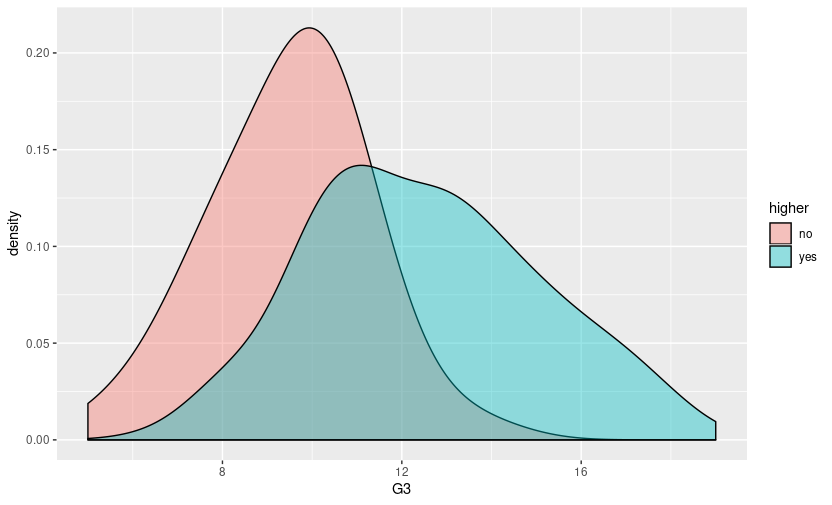
\includegraphics[width=0.6\textwidth]{pau8.png}}%
\subfigure[Boxplots]{\label{fig:b}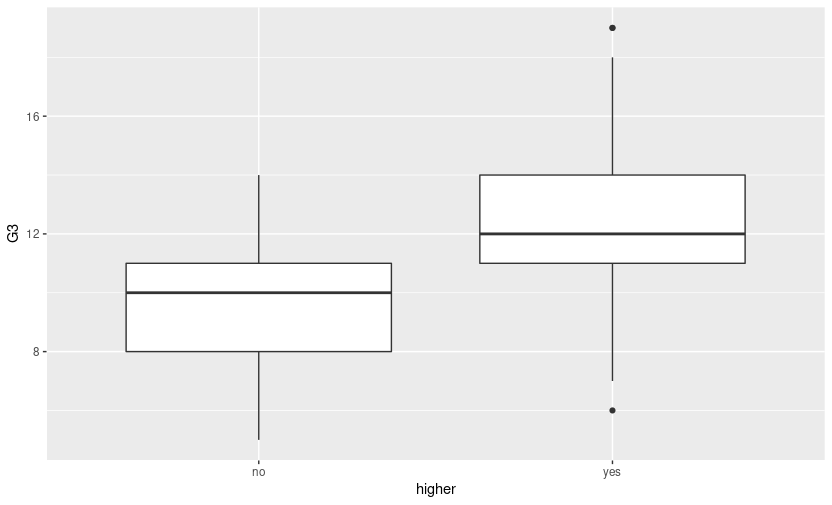
\includegraphics[width=0.6\textwidth]{pau9.png}}%
}
\end{figure*}
In these plots we can see the difference between the students that want to pursue higher education and the ones that want to enter the job market directly. In this case we can already see at first glance that there are important difference between both groups in our population. Students who want to pursue higher education tend to get higher grades than those that do not want to continue studying. In fact the first quartile of the first group coincides with the third quartile of the second group. However the medians are quite close (only 2 points difference) due to the fact that the first group is positively skewed and the second one is negatively skewed.
\newpage
Some categorical variable in our dataset take more than 2 values. In this case it is possible that there are only differences between some groups but others are similar in terms of grade distribution.\\
\begin{figure}[h]\centering
\textbf{Mother Job}\par\medskip
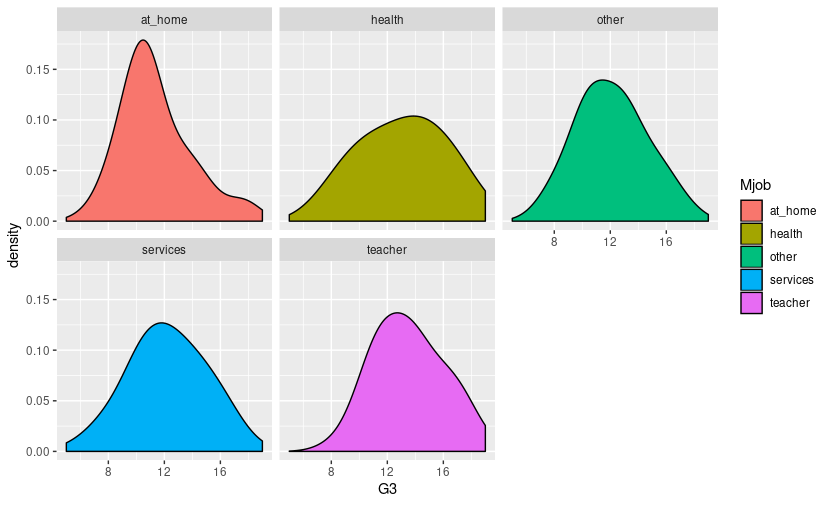
\includegraphics[width=0.9\textwidth]{pau11.png}

\end{figure}
In the figure above we can see significant differences between the smoothed densities of some groups. In fact those whose mother works either in health or education seem to be more likely to get higher grades than those in the other groups. Regarding the rest of the groups we can appreciate that the location of the distribution is very similar but they differ in terms of the tail's weight.\\
\begin{figure}[h]\centering
\textbf{Absences}\par\medskip
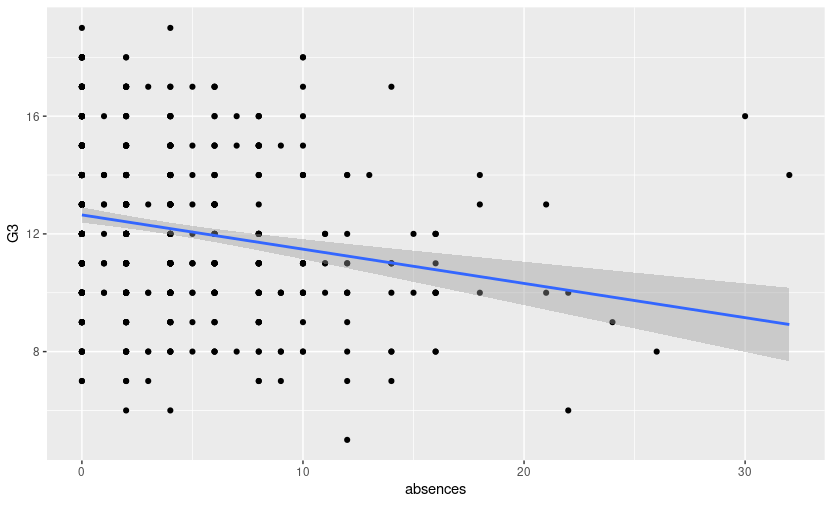
\includegraphics[width=0.9\textwidth, height = 0.3\textheight]{pau10.png}
\end{figure}
As you can see the number absences tend to have a negative impact on the final grade. However, we have to be cautious because it is not a steep slope.
\newpage
It makes perfect sense that the more absences a student has the lower the grade because the time spent in class is decreased. Nevertheless we also want to look at the relevance of the time that students spend studying in their own.
\begin{figure}[h]\centering
\textbf{Study Time}\par\medskip
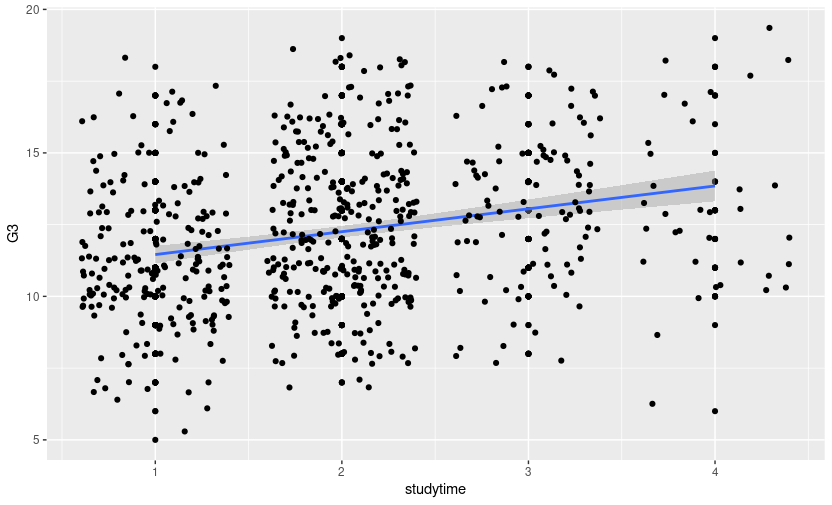
\includegraphics[width=0.9\textwidth, height = 0.3\textheight]{pau13.png}
\end{figure}
We are in the same situation as before. Despite having a trend in the data that study time contributes positively to the final grade we must be wary. In fact the slope of the fitted line is not very steep, so it could be possible that there is no statistical significance (proven in sec. 1). \\[0.3in]
\begin{figure}[h]\centering
\textbf{Mother Education}\par\medskip
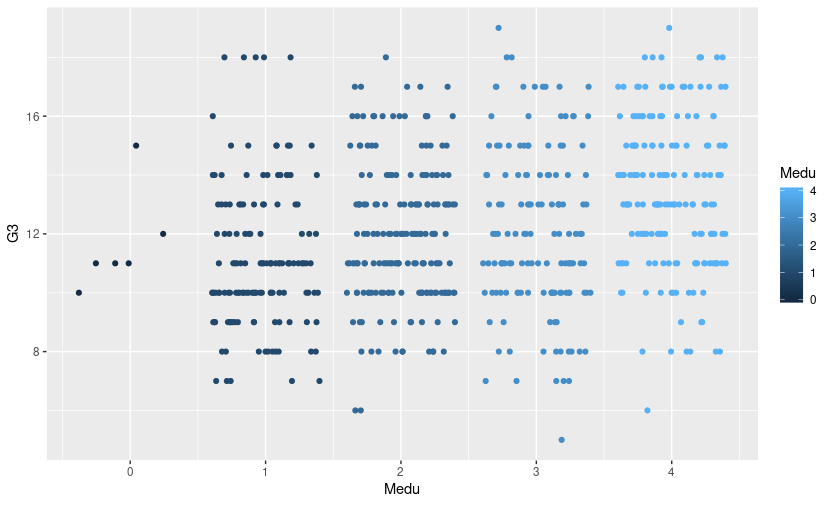
\includegraphics[width=0.9\textwidth, height = 0.3\textheight]{pau14.png}
\end{figure}
Finally we see that the level of education of the mother also seems to have a positive contribution to the final grade. Indeed, points corresponding to a higher level of education (the lighter ones) tend to have a higher G3 value.
\subsection{Data Fitting}
The goal in this section is to asses the relationship between the input variables and the final grade. Previously we have got an intuition of which are the individual effects of each explanatory variables but now we want to consider multiple inputs. In addition it is crucial to formalize our procedure beyond descriptive statistics in order to draw rigorous conclusions. We will be trying to fit a linear model of the final grade with respect to the rest of the input variables. In general terms we assume that:
$$
Y_i = \beta_0 + \beta_1X_{1i} + ... +\beta_kX_{ki} + \epsilon \quad i = 1,...,n \quad \quad \epsilon \sim \mathcal{N}(0, \sigma^2I)
$$
and want to find $\hat{\beta_0},...,\hat{\beta_k}$ that minimize the mean square error $||Y-\hat{Y}||^2$ where

$$\hat{Y_i} = \hat{\beta_0} + \hat{\beta_1}X_{1i} + ... +\hat{\beta_k}X_{ki}$$
Gauss-Markov Theorem states that under our model assumptions this estimator has the lowest sampling variance within the class of linear unbiased estimators. Now that we have exposed the theoretical aspects of our model it is time to move into practice.\\[0.3in]
First of all we want to check if our explanatory variables are useful for explaining the final grade with this model. As a result we perform an Omnibus test:
\begin{equation}
    \begin{cases}
      H_0:  & \beta_0 = \beta_1 = ... = \beta_k \\
      H_1:  & \exists j \quad  \beta_j \neq 0
    \end{cases}
  \end{equation}
  \bigskip
$$\boxed{F-statistic := 141.6 \quad \quad  p-value < 2\cdot 10^{-16}}$$
\\[0.2in]
Therefore we can reject the null hypothesis that our data is useless to predict the final grade through a linear model. Nevertheless, if we want to explain the data in a concise way it is important to remove any redundant information. At this point we are using 32 input variables so it is very likely that some of them are either irrelevant or redundant. In order to select the right variables that explain the model without redundancies we use backward selection with two factor Anova. In other words we begin with a linear model that includes all the parameters and then remove the variable with the highest p-value according to the Anova test. This test is basically a tool to quantify the marginal effect of a variable assuming the presence of the rest. Although this looks similar to what we did when testing hypothesis in section one it is important to point some differences out. In fact, when we remove a variable following this procedure we are not saying that it has no effect on the final grade. In this setting when we remove a variable we only mean that it has no effect on the final grade under the presence of the rest of the inputs. Therefore it would be wrong to say that the removed variables have no contribution to the response. Another important point to bear in mind is that at each iteration we only remove one variable even if the test outputs several variable with p-values larger than the threshold. The reason for this is that the removal of one predictor could increase the significance of another. Indeed this is what happens very often in practice.
\begin{table}[ht]
\centering
\textbf{Anova Type II}\par\medskip
\begin{tabular}{lrrrr}
  \hline
 & Sum Sq & Df & F value & Pr($>$F) \\
   \hline
G2 & 457.14 & 1 & 661.01 & 0.0000 \\
  G1 & 35.64 & 1 & 51.53 & 0.0000 \\
  age & 8.86 & 1 & 12.81 & 0.0004 \\
  failures & 4.67 & 1 & 6.76 & 0.0095 \\
  higher & 3.98 & 1 & 5.76 & 0.0167 \\
  schoolsup & 2.59 & 1 & 3.74 & 0.0535 \\
  traveltime & 2.50 & 1 & 3.61 & 0.0580 \\
  absences & 2.37 & 1 & 3.43 & 0.0646 \\
  school & 2.78 & 1 & 4.02 & 0.0454 \\
  sex & 2.57 & 1 & 3.71 & 0.0545 \\
  Residuals & 429.48 & 621 &  &  \\
   \hline
\end{tabular}
\caption{Anova test of the selected variables after the backward iterations}
\end{table}
We can see in the table above that most of the model variance is explained by the previous grades. As a result we want to test if the other variables are relevant once we already have the previous grades. We call $M_1$ the current model and $M_2$ a linear model that only includes the previous grades. Then we perform the test
\begin{equation}
    \begin{cases}
      H_0:  & M_0 \equiv M_1 \\
      H_1:  & M_0 \not\equiv M_1
    \end{cases}
  \end{equation}
    \bigskip
$$\boxed{F-statistic := 4.4639 \quad \quad  p-value =  2.8\cdot 10^{-5}}$$
\\[0.2in]
Therefore we can reject the null hypothesis, which means that the variables that we currently have in the model apart from the grades are not irrelevant at all. From now on we will stick to the model $M_1$
\newpage
\begin{center}\textbf{Goodness of fit}\end{center}\bigskip
The most widely used measure to test how well a model fits the data is the so-called coefficient of determination. It is basically the percentage of variance explained by the model.
$$
R^2 = 1-\frac{\sum(\hat{y_i}-y_i)^2}{\sum(y_i-\Bar{y})^2}
$$
In order to take into account the model complexity and avoid overfitting there is an extension of the $R^2$
usually called $R^2-adjusted$. It has the following expression:
$$\tilde{R}^2 = 1-(1-R^2)\frac{n-1}{n-p-1}$$
In our particular case both are very similar because we have already performed feature selection.
$$\boxed{R^2 := 0.9037 \quad \quad  \tilde{R}^2 =  0.9022}$$
\bigskip
\begin{center}\textbf{Collinearity}\end{center}\bigskip
We can express our linear model as $\hat{Y} = X\hat{\beta}$ and find $\beta$ such that $(X^TX)\beta = X^TY$. This is equivalent to the least square estimate, but it is not unique unless $X^TX$ is a full rank matrix. In the former case it causes many problems in terms of interpretability because the model becomes non identifiable. Then the meaning of the parameters can be misleading and this can lead us to miss the importance of some variables. In order to detect collinearity we can perform a regression of each input variable $X_i$ based on all other inputs. For each explanatory variable we will get an associated coefficient of determination $R_i^2$. We want these to be as low as possible otherwise we will increase the variance of the estimator. This leads to the concept of \textbf{Variance Inflation Factor} $\frac{1}{1-R_i^2}$
\begin{center}
\begin{tabular}{|c|c|c|c|c|}
 \hline
 \multicolumn{5}{|c|}{\textbf{Variance Inflation Factors}} \\
 \hline
 \hline
\textbf{G2} & \textbf{G1} & \textbf{age} & \textbf{failures} &  \textbf{higher} \\
\hline
 5.13 & 5.33 & 1.24 & 1.31 & 1.23 \\
 \hline
 \hline
 \textbf{schoolsup} & \textbf{traveltime} & \textbf{absences} & \textbf{school} & \textbf{sex}\\
 \hline
  1.1 & 1.08 & 1.13 & 1.24 & 1.06\\
 \hline
\end{tabular}
\end{center}
\newpage
Most authors say that variables must be removed when its VIF is higher than 5 and some suggest lower threshold values but not lower than 2. So we can proceed to remove grade 1 on our predictors to avoid collinearity. Now we can check that there is not collinearity anymore. \bigskip
\begin{center}
\begin{tabular}{|c|c|c|c|c|}
 \hline
 \multicolumn{5}{|c|}{\textbf{Variance Inflation Factors}} \\
 \hline
 \hline
\textbf{G2} & \textbf{G1} & \textbf{age} & \textbf{failures} &  \textbf{higher} \\
\hline
 1.38 & X & 1.21 & 1.30 & 1.21 \\
 \hline
 \hline
 \textbf{schoolsup} & \textbf{traveltime} & \textbf{absences} & \textbf{school} & \textbf{sex}\\
 \hline
  1.1 & 1.08 & 1.13 & 1.24 & 1.06\\
 \hline
\end{tabular}
\end{center}
\bigskip
Despite removing a variable that was highly correlated with the response we should not expect a significant deterioration in the goodness of fit.
$$\boxed{R^2 := 0.8957 \quad \quad  \tilde{R}^2 =  0.8942}$$
\bigskip
\begin{table}[ht]
\centering
\begin{tabular}{ccccc}
\hline
  & Estimate & Std. Error & t value & Pr($>$$|$t$|$) \\
  \hline
(Intercept) & 0.0415 & 0.5709 & 0.07 & 0.9420 \\
  G2 & 0.9076 & 0.0154 & 59.05 & 0.0000 \\
  age & 0.0771 & 0.0312 & 2.47 & 0.0138 \\
  failures & -0.2014 & 0.0678 & -2.97 & 0.0031 \\
  higheryes & 0.3730 & 0.1259 & 2.96 & 0.0032 \\
  schoolsupyes & -0.2614 & 0.1178 & -2.22 & 0.0268 \\
  traveltime & 0.0922 & 0.0478 & 1.93 & 0.0541 \\
  absences & -0.0152 & 0.0079 & -1.94 & 0.0532 \\
  schoolMS & -0.2495 & 0.0801 & -3.12 & 0.0019 \\
  sexM & -0.1572 & 0.0720 & -2.18 & 0.0294 \\
   \hline
\end{tabular}
\end{table}

In this figure we can see a summary of the fitted model. The first two colums contain the parameter estimates and their standard errors respectvely. The last two columns contain the information from the anova test for the marginal effect of each variable. \bigskip

The simplicity of the model makes it very easy now to interpret the results and quantify the contribution of each variable. As expected from the visualization the grade of the second semester has a high impact on the final grade. In fact, each point increase in the second term grade will increase by 0.9 the final grade. Conversely the age of the student has very little effect, but older students are more likely to get higher grades. This trend can become significant when we compare 15 year old students against 22 year-old student. The later will have on average 0.5 higher grade when all the other factors are equal. The school attended by the student can also lead to higher or lower grades but there are no big differences. The same goes for the gender that despite having some positive effect for women it is not as determinant as other factors like if the student wants to pursue higher education. Finally we have some variables with negative effect on the grade, the most important being the number of failures. Indeed we could say that a past failure has the same effect as 20 absences. The school support variable also has a negative parameter. However this does not mean that the extra education support causes a lower performance in the final exam. It could be explained by the fact that students that receive support tend to have more difficulties studying and that is the reason why they turn to the extra support.

\end{document}
